\documentclass[11pt]{article}

\usepackage[margin=1in]{geometry}
\usepackage{booktabs}
\usepackage{graphicx}
\usepackage[hidelinks]{hyperref}
\usepackage[numbers,sort&compress]{natbib}
\emergencystretch=2em

\title{Next-Observation Prediction and Delayed Clue Memory: A Controlled MiniGrid Pilot}
\author{[Author name to be supplied]}
\date{2026-10-01}

\begin{document}
\maketitle
\begin{center}
\large\textbf{EXPLORATORY WORKING DRAFT}
\end{center}

\begin{abstract}
This working draft reports a small, standalone pilot asking whether auxiliary next-observation prediction makes a recurrent memory more useful for a delayed decision. The setting is a controlled adaptation of MiniGrid Memory: a scripted, clue-independent route carries the agent from an early key/ball clue to a final forced choice, and the learned model controls only the final choice. A task-only GRU reached 100\% observed-clue success for all three training seeds. A matched GRU trained with the same task loss plus action-conditioned next-view prediction reached 50\%, 100\%, and 100\%. All never-observed clue conditions were 50\%, as expected from balanced forced choice. The predictive objective improved next-view prediction relative to the control model's untrained prediction head, but this was not reliable evidence of better decision-relevant memory. A post-hoc target audit found that after the clue disappeared, 0 of 6,336 matched next-view targets depended on clue identity. The result is best read as an optimization-sensitive exploratory pilot with a ceiling control, not as a novelty claim, a reinforcement-learning result, an LLM result, or an AgentSpec reproduction.
\end{abstract}

\section{Question and Motivation}

BeliefSpec asks: under what controlled conditions does predictive supervision make an agent's memory more useful for decisions? The mechanism tested here is deliberately small. A recurrent encoder receives partial observations and previous actions. Both learned variants train on the same supervised clue-readout objective. The predictive variant adds an auxiliary action-conditioned next-observation objective. The narrow empirical question is whether that extra predictive loss improves the final decision when architecture, data, checkpoint selection, and evaluation episodes are matched.

This pilot is motivated by, but does not claim novelty over, prior work on predictive belief states and world models. Gregor et al.\ trained belief states with generative environment-model objectives for reinforcement learning and explicitly raised the issue that prediction targets and horizons shape what information the latent state must retain \citep{gregor2019shaping}. PlaNet and Dreamer use learned latent dynamics for planning or imagined control, at a much broader scale than this supervised diagnostic \citep{hafner2019planet,hafner2020dreamer}. AgentSpec is the closest Q-Lab connection: it studies embodied-agent scaffolds through controlled composition of modules such as perception, memory, reasoning, reflection, and action \citep{chen2026agentspec,chen2026agentspec_repo}. This pilot follows the controlled-composition spirit, but it is not integrated with AgentSpec and does not reproduce its results. WorldEvolver and 3D-Belief are relevant modern examples of action-conditioned prediction or embodied belief modeling, but their representations and interfaces differ substantially from this fixed, categorical memory task \citep{zhang2026worldevolver,yin2026threedbelief}.

\section{Task and Information Access}

The experiment uses a controlled adaptation of MiniGrid Memory \citep{farama2026minigrid_memory}. The underlying simulator is MiniGrid's \texttt{MemoryEnv(size=13, random\_length=False)} with 7 by 7 egocentric object-id observations. The agent initially sees a clue object, either key or ball. A scripted controller then follows a clue-independent route through the corridor and stops at a final decision view containing two visible options. The tested method supplies only the final top/bottom choice. Thus this is not autonomous navigation, reinforcement learning, or an LLM-agent experiment.

\begin{figure}[t]
  \centering
  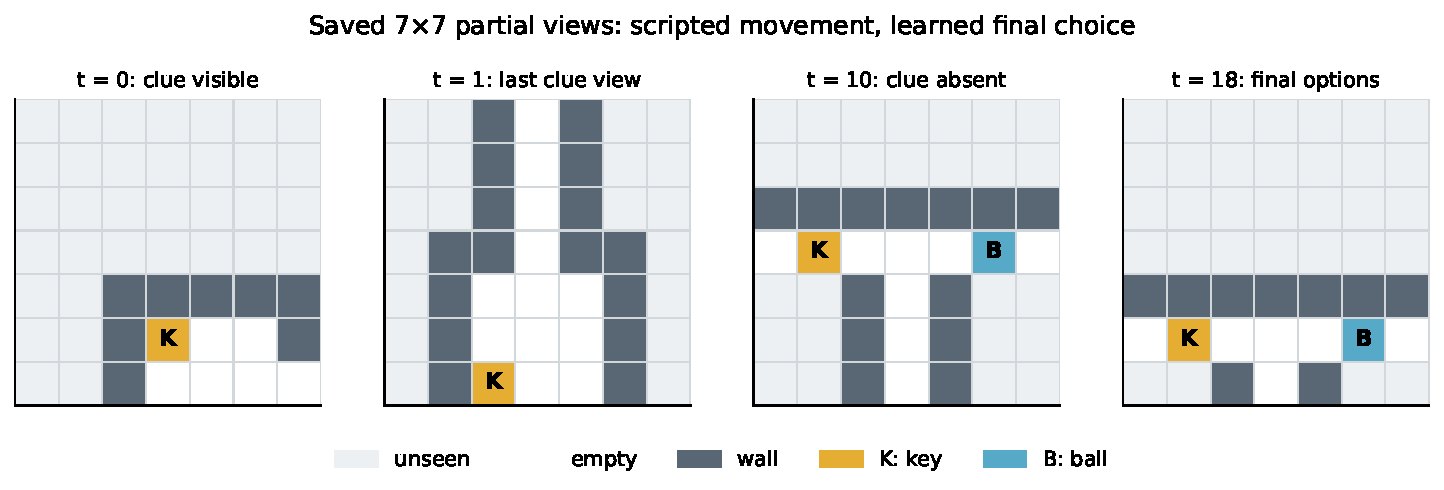
\includegraphics[width=0.86\linewidth]{../review/2026-10-01/figures/task_illustration.pdf}
  \caption{Actual saved partial observations from episode \texttt{test:test-w8-r0:h0:top0:seen}. The original clue is visible at steps 0 and 1. Later key/ball objects are choice options, not a reappearance of the original clue. The final decision at step 18 has measured delay 17.}
  \label{fig:task}
\end{figure}

The generator crosses hidden clue identity, top-option identity, clue exposure, and delay. Observed-clue delays are measured as steps since the last actual clue observation and equal 17, 29, and 53. Never-observed episodes mask the clue while it would otherwise be visible, so the correct answer is unavailable from permitted observations. Train, validation, and test splits contain 1,536, 384, and 768 episodes respectively, with zero visible-history overlap. All splits share one geometry, so this pilot makes no layout-generalization claim.

Permitted model inputs are object-id observations, direction, previous action, and a shared route phase. The object grid is encoded categorically, direction/action/phase are one-hot encoded, and the learned recurrent input dimension is 554. For the prediction head, the current executed action is also available. Mission text, filenames, seed identifiers, rewards, simulator hidden state, full-map renderings, and evaluator-only truth are excluded from model inputs. Evaluator-only logs are retained for scoring and audits.

\section{Models, Losses, and Protocol}

Six methods share a common downstream decision contract. Current-observation memory uses only the final view. Recent-history memory stores a fixed 32-record observation/action window. Structured memory stores a previously observed clue fact. Episodic retrieval returns a previously observed clue-bearing frame when one exists. The learned control model is a compact GRU trained only on the common clue-readout objective. The predictive model is the same architecture and training setup plus auxiliary next-view prediction.

The memory readout is a three-class probability vector over key, ball, and unknown. The binary controller computes the probability of choosing the top branch as $p_{\mathrm{top}} = p_{\mathrm{top\ clue}} + 0.5p_{\mathrm{unknown}}$ and chooses top when $p_{\mathrm{top}}\geq 0.5$. Three-class readout accuracy is reported separately from binary success. Task labels are the observed clue class derived from permitted history for both learned variants, with unknown when the clue is never observed. The predictive loss is categorical cross-entropy over next observation object IDs: state and action at time $t$ predict the object grid at $t+1$. The predictive arm uses task CE plus $0.1$ times prediction CE. Object IDs are categorical classes, not continuous targets.

The learned variants use encoder width 48, GRU hidden size 32, batch size 64, Adam learning rate 0.003, gradient clipping 1.0, 30 epochs, and 720 updates per run. Within each seed, control and predictive runs share initialization, minibatch order, optimizer settings, architecture, data, and checkpoint rule; only the prediction loss term is active in the predictive arm. Task loss uses each sequence's true final state; a mask excludes padded transitions from prediction loss, which is averaged over valid transitions and cells. Checkpoints are selected by minimum validation task cross-entropy with earliest tie. Seeds are 11, 22, and 33. Each run allocates 56,171 parameters: 34,611 shared encoder/recurrent/readout parameters plus a 21,560-parameter prediction head. The control run allocates the head for accounting, but only the shared 34,611 parameters are active. Therefore the control prediction metrics are an untrained comparison, not a trained predictive baseline.

The protocol was written before main training and final scoring. Validation checks covered observation/target alignment, padding masks, episode reset, gradient path, save/load equality, tiny-subset fitting, structured-memory solvability, split overlap, hidden-state leakage, simulator replay, and decoded-memory interventions. No main run was excluded.

\section{Results}

\begin{figure}[t]
  \centering
  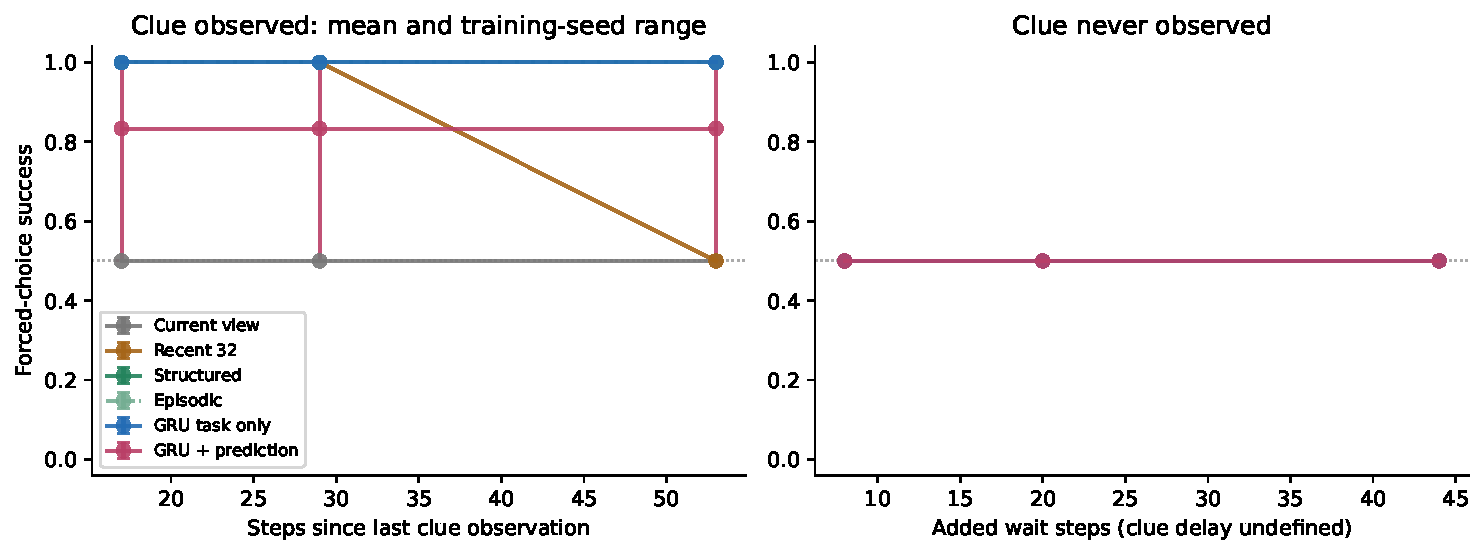
\includegraphics[width=0.88\linewidth]{../review/2026-10-01/figures/decision_success.pdf}
  \caption{Decision success by delay. Learned-method points are means across three training seeds; vertical ranges show the minimum and maximum seed values, not confidence intervals. Deterministic baselines have one value per condition. Never-observed clues have no defined clue delay, so the right panel uses added wait steps.}
  \label{fig:decision}
\end{figure}

The primary result is shown in Table~\ref{tab:seeds}. The paired seed-level predictive-minus-control differences were $-50$, 0, and 0 percentage points. The equal-delay mean difference was $-16.667$ percentage points, with sample SD 28.87 percentage points and a descriptive 95\% $t$ interval of $[-88.38, +55.04]$ percentage points using df=2. This interval is unstable and treats training seed as the unit of replication. It is not an episode-binomial confidence interval.

\begin{table}[t]
\centering
\caption{All six learned main runs. Observed success averages equally across delays 17, 29, and 53. Never-observed success is over balanced masked-clue episodes.}
\label{tab:seeds}
\begin{tabular}{llrrrr}
\toprule
Variant & Seed & Selected epoch & Observed success & Never success & Active params \\
\midrule
Control & 11 & 30 & 1.00 & 0.50 & 34,611 \\
Predictive & 11 & 10 & 0.50 & 0.50 & 56,171 \\
Control & 22 & 30 & 1.00 & 0.50 & 34,611 \\
Predictive & 22 & 30 & 1.00 & 0.50 & 56,171 \\
Control & 33 & 30 & 1.00 & 0.50 & 34,611 \\
Predictive & 33 & 30 & 1.00 & 0.50 & 56,171 \\
\bottomrule
\end{tabular}
\end{table}

The deterministic baselines behaved as intended. Current observation alone stayed at 50\% for observed clues because the clue was no longer visible at decision time. Recent history solved delays 17 and 29 but fell to 50\% at delay 53, matching the 32-record window limit. Structured memory and episodic retrieval solved all observed-clue delays and stayed at 50\% on never-observed clues.

\begin{figure}[t]
  \centering
  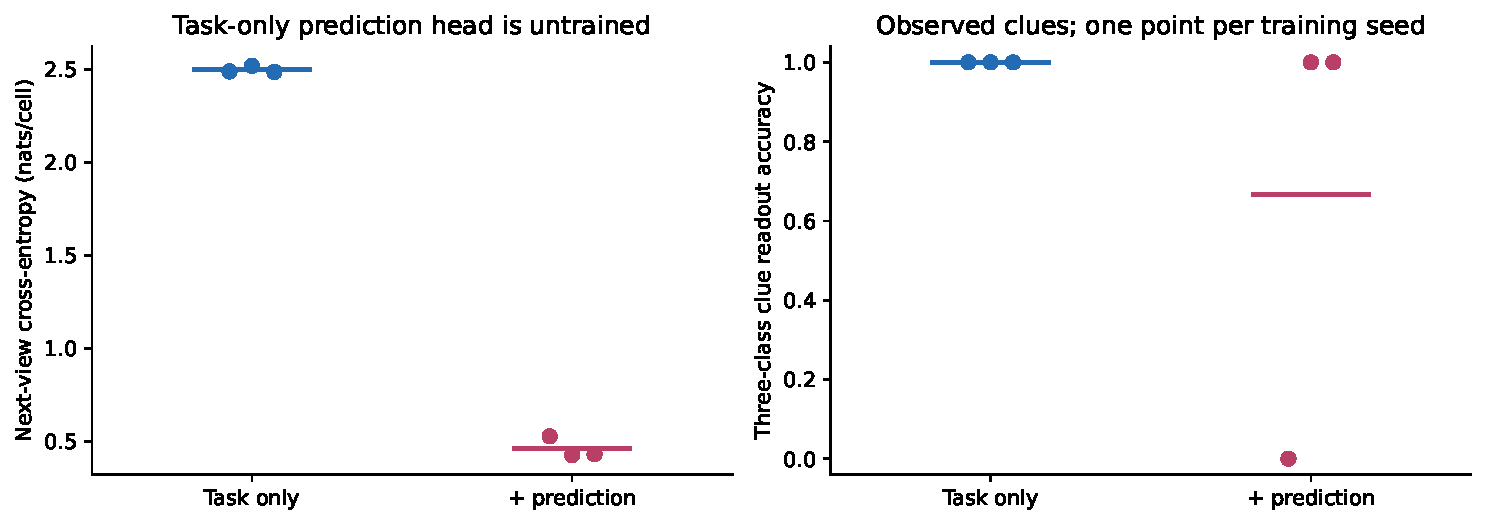
\includegraphics[width=0.88\linewidth]{../review/2026-10-01/figures/prediction_and_memory.pdf}
  \caption{Prediction and memory metrics on observed-clue episodes. Each dot is one seed's mean across delays; horizontal lines are means across seeds, not uncertainty intervals. The task-only prediction head is untrained. Predictive seed 11 achieved lower next-view CE while its clue readout remained incorrect.}
  \label{fig:predmemory}
\end{figure}

Prediction metrics separated local prediction from decision memory. On observed-clue episodes, control next-view CE/accuracy were 2.4886/0.1180, 2.5180/0.0815, and 2.4858/0.0717 for seeds 11, 22, and 33. Predictive CE/accuracy were 0.5273/0.7633, 0.4258/0.7963, and 0.4306/0.7918. Copy-current-view accuracy was 0.5999. The better predictive loss is not itself evidence of better decision memory.

\begin{figure}[t]
  \centering
  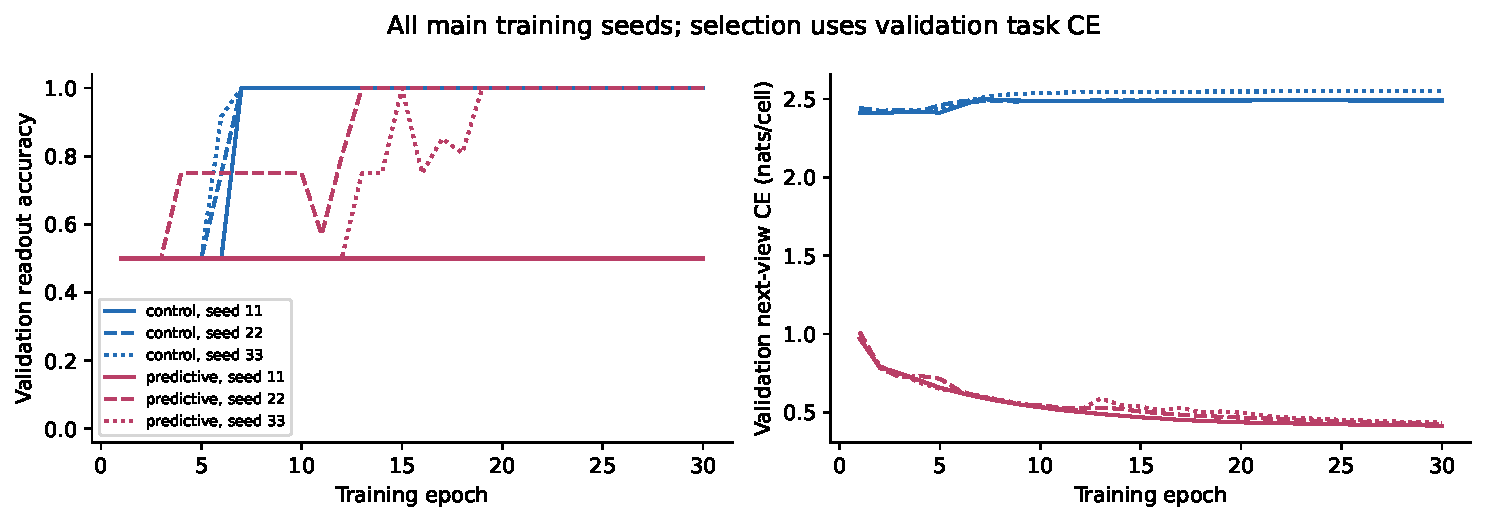
\includegraphics[width=0.88\linewidth]{../review/2026-10-01/figures/learning_curves.pdf}
  \caption{Validation learning curves by seed. Lines are individual training seeds, not uncertainty bands. Control seeds first reached at least 99\% validation readout accuracy at epoch 7. Predictive seeds 22 and 33 reached it at epochs 13 and 15. Predictive seed 11 never reached it and selected epoch 10 by the frozen validation task-CE rule.}
  \label{fig:curves}
\end{figure}

The seed-11 predictive failure was visible in readout quality. Control seeds had observed-clue and never-observed readout accuracy 1.0. Predictive seeds 22 and 33 matched that. Predictive seed 11 had observed-clue readout accuracy 0.0 and never-observed readout accuracy 1.0. In a saved failure trace, predictive seed 11 assigned probabilities $p_{\mathrm{key}}=0.2507$, $p_{\mathrm{ball}}=0.2499$, and $p_{\mathrm{unknown}}=0.4994$ at the decision point, produced an unknown readout, chose top by the deterministic interface, and failed when the hidden clue was ball and the top option was key.

\section{Post-hoc Target Audit}

The original protocol warned that one-step local prediction might not require retaining the remote clue. A post-hoc deterministic target audit made this concern concrete. Across 192 observed key/ball matched episode pairs, the only clue-dependent prediction input time was $t=0$. After the clue disappeared, 0 of 6,336 paired next-view targets differed by clue identity. This audit was not the primary experimental result and does not identify why predictive seed 11 failed. It does show that the chosen next-observation objective did not force the recurrent state to preserve clue identity over the measured decision delay.

\section{Limitations and Competing Explanations}

This pilot has several hard limits. First, the task-only GRU hit ceiling on observed clues, leaving no room to demonstrate improvement. Second, there were only three training seeds, and one predictive seed failed while two matched ceiling. Third, the fixed geometry prevents layout-generalization claims. Fourth, the prediction-head comparison in the control model is untrained, so it should not be framed as a breakthrough prediction result. Fifth, no shuffled-target placebo, duplicate-clue-loss baseline, loss-weight sweep, or longer-budget rescue run was performed.

Competing causes remain unresolved. Predictive seed 11 may reflect optimization instability, loss competition, an unlucky seed, a too-local target, or an insensitive task. The evidence does not show that predictive supervision is generally harmful. It shows that in this fixed, supervised, scripted-controller task, improved local next-view prediction was not reliable evidence of improved delayed clue memory.

\section{Proposal-only Future Questions}

\paragraph{Target relevance.} Hypothesis: a predictive target requiring delayed clue retention improves decision success relative to local prediction. Minimal change: add a future clue-dependent panel after the corridor; forecast its categorical content from the pre-reveal state and score the decision before the panel becomes an input. Use a neutral panel for never-observed histories so this custom target adds no hidden clue label. Controls: task-only GRU, local-prediction GRU, shuffled-panel-target placebo, and duplicate-clue CE that adds the same amount of direct clue supervision. Primary metric: paired seed-level decision success on a development-calibrated non-ceiling task; readout accuracy and panel CE are supporting metrics. Counterevidence: panel prediction improves but decisions do not. Remaining alternatives: extra supervision, easier gradients, duplicated clue labels, or regularization rather than a predictive mechanism. This is the first priority because it directly tests the pilot's target-relevance limitation.

\paragraph{Information gathering.} Hypothesis: a memory-conditioned observation action improves decisions when clue information is absent or unreliable. Minimal change: before the final choice, allow \emph{inspect} (a reliable clue-refresh observation at a known cost) or \emph{commit}. Controls: always inspect, never inspect, an observation-based confidence-threshold policy, and matched task-only/predictive query policies, all charged the same cost. Primary metric: mean decision success minus inspection cost; query rates on sufficient versus insufficient histories are supporting measures. Counterevidence: no utility gain over fixed policies, or indiscriminate querying. Remaining alternatives: the cost may make one fixed policy optimal, or calibration and direct query supervision may explain the gain without predictive memory.

\paragraph{Adaptation.} Hypothesis: a recurrent state can retain valid clues but revise its clue estimate and uncertainty when the world changes. Minimal change: a later visible event either confirms the clue, reveals a replacement, or signals invalidation without revealing the replacement. Keep the key/ball/unknown contract; unavailable replacement identity is unknown, not a hidden training label. Controls: initial-clue-only memory, latest-supported-fact memory, recency memory, and matched task-only/predictive GRUs. Primary metric: decision success by unchanged, replacement-observed, and invalidated-only conditions; unknown readout and calibration support the uncertainty analysis. Counterevidence: stale choices persist, valid old clues are discarded, or unsupported confidence remains after invalidation. Remaining alternatives: recency, an explicit phase marker, direct update labels, or an easy-to-parse late cue may suffice without richer belief maintenance.

None of these proposals was executed. Each requires its own protocol, fresh training seeds and held-out trajectories, and development-only difficulty/budget selection before final evaluation. Recognizing unknown in the current pilot is not evidence of calibrated uncertainty, active information gathering, or continual adaptation.

\section{Reproducibility and Contribution Statement}

The main runs completed locally on macOS 15.7.7 arm64, CPU only, two Torch threads, 16 GiB physical memory. Original main-training logs report six runs in 109.224 seconds total wall time, with peak macOS RSS 576,798,720 bytes. Package checks verified 50 frozen files, 7,680 episode rows, 1,920 hidden-swap output checks, 768 simulator replays, 30,720 intervention rows, and exact fresh-environment reproduction for control seed 11. An independent review audit under \texttt{review/2026-10-01/verification/} confirmed the same split counts, zero split overlap, seed results, checkpoint-selection matches, and exact control-seed-11 reproduction. The review rerun recorded 22 passing tests in 4.06 seconds.

Original timings were 14.8--15.4 s per task-only run and 20.9--21.3 s per predictive run. Recorded inference took 0.153--0.180 s per learned checkpoint over 768 episodes, excluding simulator replay; these are individual timings, not a hardware benchmark. New review inference also matched all six saved checkpoints' probabilities and prediction metrics to the raw records, with zero differences.

Raw results are in \path{results/final/episodes.csv}; original run metadata are in \path{artifacts/main_execution.json}; new checks are in \path{review/2026-10-01/verification/public_audit_final.json}; and regenerated figures are under \path{review/2026-10-01/figures/}. Private application drafts and personal-path logs are excluded from the public package. No email, form submission, or preprint upload was performed.

This manuscript source is an AI-assisted working draft prepared from the saved BeliefSpec package. The author identity and personal contribution statement are placeholders and must be finalized before scholarly submission. The experimental package itself records AI-assisted engineering and documentation support; this draft should be treated as a review artifact, not as a claim of independent unaided work.

\bibliographystyle{plainnat}
\bibliography{references}

\end{document}
